\documentclass{apuntes}
\newcommand{\acum}[1]{\#1 \subset(#1) }
\usepackage{tikz}
\title{Análisis Matemático}
\author{Víctor de Juan Sanz}
\date{13/14 C1}
\usetikzlibrary{arrows}
\begin{document}
\maketitle
\newpage
\tableofcontents
\newpage
Datos de interés:\\
Jesus Garcia Azorero\\
Despacho: 17-608\\
Correo: jesus.azorero@uam.es


\section{Contenido de la asignatura}
\subsection{Preliminares}
Repaso de contenidos de Cálculo II como conjuntos abiertos y cerrados, gradiente \dots
\subsection{Teorema funcion inversa, implicita y rango}
Aplicación a funciones no lineales de los teoremas fundamentales de cálculo II
\subsection{Mínimos y máximos condicionados}
Multiplicadores de Lagrange
\subsection{Subvariedades diferenciales}
Objetos de dimensión n en espacios de dimensión m ($n<m$).
\subsection{Integración en subvariedades diferenciales}
\subsection{Teorema de Stokes}
Demostración del teorema con lenguaje de las formas diferenciales.
\newpage


\section{Preliminares del análisis matemático}
A lo largo del curso vamos a trabajar en $\real^n={(x_1,\dots c, x_n) \  x_j \in \real, j=1,...,N}$
\subsection{Producto escalar, norma y distancia}
Durante todo el año denotaremos al vector $(x_1,x_2,\dots,x_n)$ como $\gx$ por comodidad.

\begin{defn}[Producto escalar euclídeo]

\[ \pesc{\gx,\gy} = \sum_{i=1}^{N} x_iy_i \]


Propiedades:
\begin{itemize}
 \item $\pesc{\lambda \gx, \gy} = \lambda \pesc{\gx, \gy}$
 \item $\pesc{\overline{x} + \overline{y}, \overline{z}}= \pesc{\gx+\gz}+\pesc{\gx,\gy}$
 \item $\pesc{gx, \gy} = \pesc{\gy,\gx}$
 \item $\pesc{\gx, \gx} ≥ 0$
 \item $\pesc{\gx,\gx} = 0 \implies \gx = \gor{0}$
\end{itemize}

Las tres primeras son la consecuencia de que el producto escalar tiene que ser bilineal.
\end{defn}

En general, un producto escalar es una matriz definida positiva y se opera de la siguiente manera:

\[\pesc{\gx,\gy} = (x_1,x_2,...,x_N) \cdot \begin{pmatrix}
a_11 &\cdots& a_1N\\ 
\vdots& \ddots & \vdots\\
a_N1 & \cdots& a_NN
\end{pmatrix}
\cdot \begin{pmatrix} y_1\\
																				\vdots\\ y_N \end{pmatrix}\]


\begin{defn}[Norma\IS euclídea]

\[ \md{\gx} = \left(\pesc{\gx,\gx}\right)^{\frac{1}{2}} = \dotsb = \left(\sum_{i=1}^{N}x_i^2\right)^{\frac{1}{2}} \]
Propiedades:
\begin{itemize}
 \item  $\md{\gx} = 0 \dimplies \gx = 0$
 \item	Homogeneidad: $\md{\lambda\gx} = \lambda\md{\gx}$
 \item	Desigualdad triangular: $\md{\gx+\gy} \leq \md{\gx}+\md{\gx}$
\end{itemize}

\end{defn}


\begin{lemma}
$\md{\gx} = (\gx * \gx) ^ \frac{1}{2}$ para cualquier producto escalar $*$.
\end{lemma}


\begin{defn}[Norma]
Cualquier operación que cumpla las 3 propiedades anteriores es una \textbf{norma}.

En general se tiene $\md{\cdot}_p, p \in \mathbb{N}$ y se definen todas de la misma forma:

\[ \md{\gx}_p = \left(\sum_{i=1}^N |x_i|^p \right)^\frac{1}{p} \]

\end{defn}

Hay tres casos particulares, la norma uno \index{Norma!uno}
\[ \md{\gx}_1 = |x_1| + |x_2| + ... + |x_n| \]

La norma 2, que es la norma euclídea

y la norma infinito \index{Norma!infinito}
\[\md{\gx}_{\infty} = \max\left\{|x_1|,|x_2|,\dots,|x_n|\right\} \]

 Vamos a demostrar que la norma $p$ cumple las 3 propiedades de una norma. Para ello, nos apoyaremos en dos teoremas previos:

\begin{theorem}[Desigualdad\IS de Young]
 Sea $p > 1$ y tomamos $p'$ tal que $\frac{1}{p}+\frac{1}{p'} = 1$ (exponente conjugado). Entonces:

\[ |ab| \leq \frac{1}{p} \cdot |a|^p +\frac{1}{p'} |b| ^ {p'} \]
\end{theorem}
 
\begin{proof}
Se utiliza la idea de la función logaritmo, que es cóncava\footnote{Geométricamente, cóncava significa que si uno 2 puntos de la gráfica, la recta que los une queda debajo de la gráfica.} y creciente.  Tomando 2 puntos $A$ y $B$ tenemos la condición de concavidad 

\[ t \log A + (1-t) \log B \leq \log (tA + (1-t) \cdot B)\]

. Utilizando la derivada hallamos la ecuación de la recta que pasa por $A$ y por $B$ y tomamos un punto que dista $t$ de $A$ y $(1-t)$ de $B$. Como la función es cóncava sabemos que ese valor será menor que el valor del logaritmo en un punto $t$ entre $A$ y $B$.

Tomando $A=|a| ^ p$, $B = |b| ^ p$ y $t = \frac{1}{p} \rightarrow 1-t = \frac{1}{p'}$ tenemos que

\begin{align*}
\frac{1}{p}\cdot log |a|^p + \frac{1}{p'} \cdot log|b|^{p'} &\leq log\left(\frac{1}{p}|a|^p + \frac{1}{p'} |b|^{p'}\right) \\
\log \abs{a} + \log \abs{b} &\leq log\left(\frac{1}{p}|a|^p + \frac{1}{p'} |b|^{p'}\right) \\
\log \abs{ab} &\leq log\left(\frac{1}{p}|a|^p + \frac{1}{p'} |b|^{p'}\right) \\
\abs{ab} &\leq \frac{1}{p}|a|^p + \frac{1}{p'} |b|^{p'} 
\end{align*}

\end{proof} 
\begin{theorem}[Desigualdad\IS de Hölder] Se trata de una generalización de la desigualdad de Cauchy-Schwarz, que ocurre en el caso $p=2$
\[ \sum_{i=1} ^ N \abs{x_i y_i} \leq \md{\gx}_p \md{y_i}_p \]

\label{thmHolder}
\end{theorem}

\begin{proof} Tomamos  
 \begin{align*}
 a_i &= \frac{\abs{x_i}}{\md{\gx}_p} \\
 b_i &= \frac{\abs{y_i}}{\md{\gy}_{p'}}
 \end{align*}
 
 Tenemos que \[ a_i b_i \leq \frac{1}{p}a_i ^ p + \frac{1}{p'} b_i^{p'} \]
 
 Sustituimos: 
 \[  frac{\abs{x_i}}{\md{x}_{p}} \cdot \frac{\abs{y_i}}{\md{y}_{p}} \leq \frac{\abs{x_i}^p}{p\cdot \md{x}_{p}^p} + \frac{\abs{y_i}^{p'}}{p'\cdot\md{y}_{p'}^{p}} \]
 
 Tomamos sumatorios y, teniendo en cuenta que $\md{x}_{p}^p = \sum|x_i|^p$, nos queda 
 
 \[ \frac{1}{\md{x}_{p}\md{y}_{p'}}\cdot \sum_{i=1}^N |x_iy_i| \leq \frac{1}{p\md{x}_{p}^p} \sum |x_i|^p + \frac{1}{p'\md{y}_{p'}^{p'}} \sum |y_i|^{p'} = \frac{1}{p} + \frac{1}{p'} = 1 \]
 
 \end{proof}
 
Una vez probadas las dos desigualdades anteriores, pasamos a probar la desigualdad triangular: 
 
\begin{proof} El objetivo es demostrar que \[ \md{\gx+\gy}_p \leq \md{\gx}_p+\md{\gy}_p \] y vamos a hacerlo en varios pasos.
 
 Para evitarnos las raíces empezamos con $\md{\gx+\gy}_p^p$

 \begin{gather*}
 \md{\gx+\gy}_p ^ p = \sum_1 ^ N |x_i+y_i| ^ p = \sum_ 1 ^ N |x_i+y_i| \cdot |x_i+y_i| ^ {p-1} =\\
 = \sum_1 ^ N |x_i|\cdot|x_i+y_i| ^ {p-1} + \sum_1^N |y_i| \cdot |x_i+y_i|^{p-1}
 \end{gather*}

 Utilizando la desigualdad de Hölder (\ref{thmHolder}) tenemos:
 
 \begin{multline*} \md{\gx+\gy}_p ^ p \leq \\
 \sum \left(|x_i|^p\right)^{\frac{1}{p}} \cdot \underbrace{\sum \left(\left(|x_i+y_i|^{p-1}\right)^{p'}\right)^{\frac{1}{p'}}}_* +
 \sum \left(|y_i|^p\right)^{\frac{1}{p}} \cdot \underbrace{\sum \left(\left(|X_i+y_i|^{p-1}\right)^{p'}\right)^{\frac{1}{p'}}}_* 
 \end{multline*}
 
 Por ser $p$ y $p'$ exponentes conjugados es fácil comprobar que $1-\frac{1}{p'} = \frac{1}{p}$\\
 Sacamos factor común y pasamos al otro lado obteniendo (PASO INTERMEDIO?)
\[ \left(\sum_1^N |x_i+y_i|^p\right)^{\overbrace{\left(1-\frac{1}{p'}\right)}^p} = \md{\gx+\gy}_p \leq \md{x}_{p} + \md{y}_{p} \]

\textit{Guille: esta demostración es muy, muy rara.}
\end{proof}


EJERCICIO PROPUESTO: Tomamos en el plano el conjunto de los puntos cuya norma es 1. Tomando en la norma p=2 sale la circunferencia. ¿Y en p=3? 


\begin{remark} Estos argumentos se pueden utilizar para demostrar
\[ \int \abs{f\cdot g}\, dx \leq \left(\int\abs{f}^p\, dx\right) ^ \frac{1}{p} \cdot \left(\int\abs{g}^{p'}\,dx\right)^\frac{1}{p'} \]
\end{remark}

\newpage


\begin{defn}[Distancia\IS euclídea]
\[d(\gx,\gy) = \md{\gy - \gx} \]
\end{defn}

Propiedades:
\begin{itemize}
 \item La distancia es siempre positiva: $d(\gx,\gy)\ge 0$
 \item $d(\gx,\gx) = 0$
 \item Simetría: $d(\gx,\gy) = d(\gy, \gx)$
 \item Desigualdad triangular $d(\gx,\gz) \leq d(\gx,\gy) + d(\gy,\gz)$. La distancia entre 2 puntos es menor o igual en línea recta que pasando por un punto intermedio.
\end{itemize}


\begin{defn}[Distancia] Cualquier operacion que cumpla las 3 propiedades anteriores es una distancia. \end{defn}

\paragraph{Recapitulando}
Con un producto escalar puedo definir una norma y con esa norma puedo definir una distancia. Pero... ¿Podemos definir una norma 
que no venga de un producto escalar y/o alguna distancia que no provenga de una norma? Sí, por ejemplo

\[ \tilde{d} (\gx,\gy) = \abs{\arctg(y) - \arctg(x)} \] 

No cuesta mucho comprobar que cumple las 3 propiedades de una distancia. Además, esta distancia es cuanto menos curiosa porque nunca será mayor de $\pi$.

 Podemos comprobar que si existiera una norma que midiese esta distancia tendríamos \[\tilde{\md{\gx}} = \tilde{d} (\gx,\gor{0}) = \abs{\arctg (x)} \]
 pero esto no cumple la propiedad: $\tilde{\md{\lambda x}} = \abs{\arctg \lambda x} \neq \abs{\lambda}\abs{\arctg x} = 
 \abs{\lambda x}\tilde{||x||}$
 ya que ninguna distancia puede ser mayor que $\pi$ y tomando un $\lambda > \pi$ se produciría la contradicción.

\subsection{Relación norma - producto escalar}
\label{secNormaprodEsc}
\begin{theorem}
Supongamos que tengo un producto escalar $\ast$ y una norma asociada \[ \md{\gx} = (\gx\ast \gx) ^ {\frac{1}{2}}\]. Entonces \[ \md{\gx + \gy}^ 2 =  \md{\gx} ^ 2 + \md{\gy} ^ 2+2(\gx\ast\gy) \]
\end{theorem}

\begin{proof}
\[ \md{\gx+\gy}^2 = (\gx+\gy)\ast(\gx+\gy) = \gx \ast \gx + \gx \ast \gy + \gy \ast \gx + \gy \ast \gy=\md{\gx} ^ 2 + \md{\gy} ^ 2+2(\gx\ast\gy) \]
\end{proof}

Esa norma asociada al producto escalar tiene dos propiedades importantes:
\begin{itemize}
\item Paralelogramo: $\md{\gx+\gy}^ 2 + \md{\gx-\gy} ^ 2 = 2\left(\md{x}^2+\md{x}^2\right) $
\item Polarización: $\md{\gx+\gy} ^ 2 - \md{\gx-\gy} ^ 2 = 4(\gx*\gy)$
\end{itemize}


\subsection{Equivalencia de normas}
Sea $\md{\cdot}$ una norma en $\real^N$. Si intento calcular la norma de un vector $\gx$

\[ \md{\gx} = \md{\sum x_i e_i} \leq \sum_{i=1}^N \md{x_1 e_1} = \sum_{i=1}^N|x_i|\cdot\md{e_i} \]

Tenemos: $\md{\gx} \leq \sum_{i=1}^N c_i |x_i|$ siendo $c_i = \md{e_i}$. Aplicando Cauchy-Schwarz  nos queda
\[ \sum_{i=1}^N \left(c_i^2\right)^\frac{1}{2} \cdot \sum \left(|x_i|^2\right)^\frac{1}{2} \]
Es decir, puedo controlar cualquier norma con una constante y la norma euclídea:
$$|||\gx||| \leq C \md{x}_{2}$$
En particular, $0 \leq |||\gor{x_n} - \gx|||\leq c ||\gor{x_n}-\gx||$. 

\begin{remark}
Si aplicamos Holder en vez de Cauchy, sale la igualdad con la norma p y no con la euclídea.
\end{remark}

\paragraph{Aplicación:}
Sea $F(\gx) = |||\gx|||$ y $F:\real^N \rightarrow \real^N$ 
$$|F(\gx)-F(\gy)| = \left| |||\gx - \gy||| \right| = |||\gx - \gy||| \leq C ||\gx - \gy||$$
Utilizando: $|||\ga-\gb||| \ge |||\ga||| - |||\gb|||$ \footnote{(la desigualdad triangular con restas, que se saca con un simple cambio de variable)}

Es decir, cualquier norma en $\real^n$ es \textbf{continua} respecto de la norma euclídea. \footnote{Continua si la tomas como una función de $\real^N$ en $\real$}

\begin{theorem}[Relación norma $\leftrightarrow$ producto escalar]
$\md{\cdot}$ una norma cualquiera de $\real^N$ proviene de un producto escalar si y sólo si la norma satisface la identidad del paralelogramo. 
\end{theorem}

\begin{proof}
En el apartado anterior (\ref{secNormaprodEsc}) demostramos la implicación hacia la derecha. Vamos a demostrar la recíproca:
Suponemos que la norma satisface la identidad del paralelogramo:

\begin{equation}
 \md{\ga+\gb}^2 + \md{\ga-\gb}^2 = 2 \md{\ga}^2 + 2\md{\gb}^2 \label{eqParalelogramo}
\end{equation}
Queremos probar que existe un producto escalar $\ast$ tal que $\md{\gx} = (\gx\ast \gx)^\frac{1}{2}$, así que definimos uno utilizando la identidad de polarización: 

\begin{equation}
 \gx\ast\gy = \frac{1}{4} \left( \md{\gx+\gy} ^ 2 - \md{\gx-\gy} ^ 2\right) \label{eqPolarizacion}
 \end{equation}

Queremos probar que, efectivamente, $\ast$ es un producto escalar, así que tenemos que demostrar las siguientes propiedades:
\begin{enumerate}
 \item $\gx\ast\gy = \gy\ast\gx$ .
 \item $\gx\ast\gx \ge 0\quad \forall\; \gx$
 \item $(\gx\ast\gx) = 0 \dimplies \gx=\gor{0}$ 
 \item $(\lambda \gx) \ast \gy = \lambda\left(\gx\ast\gy\right)$
 \item $(\gx+\gy)\ast\gz =\gx\ast\gx + \gy\ast\gz $
\end{enumerate}

Las propiedades 1, 2 y 3 son triviales. Vamos con 4 y 5

\paragraph{Demostración de la 4ª propiedad}

Demostraremos que se cumple por inducción cuando $\lambda\in\nat$. Primero probamos para $\lambda = 2$.

\begin{align*}
(2\gx)\ast\gy = && \text{usando (\ref{eqPolarizacion})} \\
= \frac{1}{4} \left(|||2\gx+\gy |||^2 - |||2\gx-\gy |||^2\right) = && \\
= \frac{1}{4} \left(|||\underbrace{\gx}_a + \underbrace{\gx+\gy}_b|||^2 - |||\underbrace{\gx}_a+\underbrace{\gx-\gy}_{-b}|||^2\right) = && \text{usando (\ref{eqParalelogramo})} \\
= \frac{1}{4} \left(2|||\gx|||^2 + 2|||\gx + \gy|||^2\right) = && \\
= 2 \frac{1}{4} \left(|||\gx+\gy|||^2 - |||\gx-\gy|||^2\right) = 2 (\gx\ast\gy) &&
\end{align*}

Conclusión: si $\lambda = 2$ vemos que sale fuera y por lo tanto se cumple.

Paso 2 de la inducción: buscamos demostrar la propiedad con $\lambda = n$ con $n \in \mathbb{N}$

\begin{align*}
(n\gx)\ast\gy = && \text{usando (\ref{eqPolarizacion})} \\
= \frac{1}{4} \left(|||n\gx+\gy|||^2 - |||n\gx-\gy|||^2\right) = && \\
= \frac{1}{4} \left(|||\underbrace{(n-1)\gx}_a+\underbrace{\gx+\gy}_b|||^2 
		- ||| \underbrace{(n-1)\gx}_a+ \underbrace{\gx-\gy}_b|||^2\right)= && \text{usando (\ref{eqParalelogramo})} \\
=...=2(\gx\ast\gy) + (n-2)(\gx\ast\gy) = && \text{usando hip. de inducción}\\
= n (\gx\ast\gy)
\end{align*}

Queda demostrado por lo tanto para $\lambda \in \nat$. Falta ahora demostrarlo para el resto de conjuntos de números.

\textbf{Para $\lambda \in \ent$} utilizaremos $(-\gx) \ast \gy = - (\gx\ast\gy)$ y podremos usar la demostración de los naturales.

\textbf{Para $\lambda = n \in \rac$} con $n = \frac{p}{q}$, siendo $p$ y $q$ primos entre sí, vemos que 

\[ \left(\frac{p}{q}\gx\right)\ast\gy = \frac{q\left(\left(\frac{p}{q}\gx\right)\ast\gy\right)}{q} = \frac{\left(q\cdot\frac{p}{q}\gx\right)\ast\gy}{q} = \frac{\left(p\gx\ast\gy\right)}{q} \] que tal y como habíamos demostrado antes es igual a $ \dfrac{p\left(\gx\ast\gy\right)}{q} $, con lo que queda demostrado también para los racionales.

Por último, queremos demostrarlo cuando $\lambda \in \real$

$\lambda = \liminf{n} r_n$. Utilizaremos el resultado previo de que cualquier norma es continua.

$\gx, \gy$ fijos.

Revisar: Los $|||r_n \gx + \gy|||^2$ y  $|||r_n \gx - \gy|||^2$ son continuos.
$$\alpha \gx*\gy = \frac{1}{4}\left(||r_n \gx + \gy|||^2||| -|||r_n \gx - \gy|||^2||| \right) =$$
$$\lim_{n\to\infty} \left(||r_n \gx + \gy|||^2||| -|||r_n \gx - \gy|||^2||| \right) = \lim_{n\to\infty} (r_n\gx*\gy) = $$
$$\lim_{n\to\infty} r_n(\gx*\gy) = \alpha (\gx*\gy)$$

WTF es esto.

\paragraph{Demostración de la 4 propiedad:}
$$A = (\gx+\gy)*\gz = \frac{1}{4} \left( |||\gx+\gy+\gz|||^2 - |||\gx+\gy-\gz|||^2\right)$$
$$B =\gx*\gz = \frac{1}{4} \left( |||\gx+\gz|||^2 - |||\gx-\gz|||^2\right)$$
$$C =\gy*\gz = \frac{1}{4} \left( |||\gy+\gz|||^2 - |||\gy-\gz|||^2\right)$$
Demostraremos que $A-B-C=0$\\
COMPLETAR la comprobación.
\end{proof}
\begin{remark}
$d(\gx,\gy) = |||\gx-\gy||| \text{ para alguna norma }|||\cdot||| \dimplies (d(\gx+\gz)+d(\gy+\gz) = d(\gx,\gy) \wedge d(\lambda \gx,\lambda \gy = \abs{\lambda} d(\gx,\gy))$
\end{remark}

\section{Topología}
\begin{defn}[Bola] Se define la bola de radio $R$ centrada en el punto $\gx_0$ como 
\[B_R(\gx_0) =\{\gx \in \real^N \tq \underbrace{d(\gx,\gx_0)}_{=\md{\gx-\gx_0}} < R \} \]
\end{defn}


Para evitar jaleos, al tratar la distancia vamos a tomar la norma euclídea. Como todas las normas son equivalentes, nos da igual tomar una que otra.
\begin{defn}[Conjunto\IS abierto] Un conjunto $A \subset \real^N$ es abierto si y sólo si $\forall\, \ga\in A\; \exists \varepsilon > 0 \tq B_\varepsilon(\ga) \subset A$
\end{defn}

\begin{defn}[Conjunto\IS cerrado] Un conjunto $B \subset \real^N$ es cerrado si y sólo si su complementario $B^c= \real^N-B$ es abierto.
\end{defn}

\begin{theorem}[Caracterización de cerrados en términos de sucesiones][Caraceterización!por cerrados] Un conjunto $B \subset \real^N$ es cerrado si y sólo si para cualquier sucesión convergente $\{x_n\} \subset B$ se cumple que  $\lim x_n \in B$. 
\end{theorem}

\begin{theorem}[Operaciones con conjuntos abiertos y cerrados][]
Suponemos conjuntos de dimensión finita:
\begin{itemize}
 \item Unión arbitraria de abiertos $\rightarrow$ abierto
 \item Intersección finita de abiertos $\rightarrow$ abierto
 \item Union finita de cerrados $\rightarrow$ cerrado
 \item Intersección arbitraria de cerrados $\rightarrow$ cerrado
\end{itemize} 
\end{theorem}

\begin{defn}[Punto\IS de acumulación]
La idea intuitiva es aquellos puntos a los que puedo llegar en el límite, es decir, puntos que a su alrededor a una distancia arbitrariamente pequeña existen otros puntos del conjunto.
\[ A\subset \real^N,\; a \in (A) \dimplies  \forall \varepsilon > 0\; (B_{\varepsilon} (a) \setminus \{a\}) \cap A \neq \emptyset \]
Siendo $(A)$ es el conjunto de los puntos de acumulación.
\end{defn}

\begin{defn}[Frontera]
La frontera $∂A$ de un conjunto $A$ son aquellos puntos para los que en su entorno (para cualquier $\varepsilon$) hay puntos tanto del conjunto como puntos de fuera del conjunto.
\[ a \in ∂A \dimplies \forall \varepsilon>0 \tq B_\varepsilon (a) \cap A \neq \emptyset \y B_{\varepsilon} (a) \cap A^C \neq \emptyset \]
\end{defn}

\begin{defn}[Interior] El interior es el conjunto abierto más grande que está contenido en el conjunto $A$.\end{defn}
\begin{defn}[Cierre] El cierre de un conjunto $A$A es el conjunto cerrado más pequeño en el que está contenido $A$.\end{defn}

\begin{remark}
Cierre e interior no los vamos a definir formalmente porque se dan por supuesto.
\end{remark}

\begin{defn}[Conjunto\IS compacto]
Un conjunto que cumpla cualquiera de las 3 propieda-\\des siguientes.
\end{defn}

\begin{theorem}[Conjunto\IS cerrado y acotado]
Sea $K \subset \real^N$. Son equivalentes:
\begin{enumerate}
 \item \label{propCerrado} K cerrado y acotado.
 \item \label{propSucesion} Para cualquier sucesión $\{x_n\} \subset K$, podemos encontrar una subsucesión convergente $\{x_{n_j}\} \subset\{x_n\}$ con $\lim x_{n_j} \in K$.
 \item \label{propRecubrimiento} Dado cualquier recubrimiento $\{A_i\}$ abierto de modo que $K \subset \cup \{A_i\}$ puedo encontrar un recubrimiento finito $\{A_j\}, j=1,...,M \tq K \subset \bigcup_{i=1}^M A_i$
\end{enumerate}
\end{theorem}

\begin{proof}

\paragraph{2 implica 1}  Supongamos que $K$ no estuviera acotado (negamos la propiedad \ref{propCerrado}). Consideremos una sucesión de vectores $\{x_n\}$ de tal forma que $\md{x_n} = n$, creciente y no acotada, pero con todos los elementos en $K$. Es imposible encontrar una subsucesión convergente, lo que contradice \ref{propSucesion}.

Si, por otra parte, $K$ no fuera cerrado, tendríamos que la frontera está fuera del conjunto, y podemos encontrar una sucesión $\{x_n\}$ con $\lim x_n \in ∂K$, lo que contradice \ref{propSucesion}.

\paragraph{1 implica 2} Empecemos por el caso sencillo, explorando una sucesión cualquiera $\{\gx_n\} \subset K \subset \real$, donde $K$ es, como decíamos en el enunciado, cerrado y acotado. Para encontrar una subsucesión convergente, usaremos el criterio de bisección.

\begin{center}
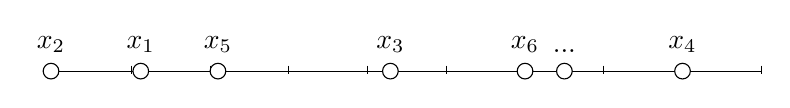
\begin{tikzpicture}
% a straight line segment
\draw (1,0) -- (10,0);
\foreach \x  in {1,...,10}
  \draw[xshift=\x cm] (0pt,2pt) -- (0pt,-1pt);
% the labels
\node[fill=white,draw=black,circle,inner sep=2pt,label=above:{$x_1$}] at (2.12,0) {};
\node[fill=white,draw=black,circle,inner sep=2pt,label=above:{$x_2$}] at (0.98,0) {};
\node[fill=white,draw=black,circle,inner sep=2pt,label=above:{$x_3$}] at (5.29,0) {};
\node[fill=white,draw=black,circle,inner sep=2pt,label=above:{$x_4$}] at (9,0) {};
\node[fill=white,draw=black,circle,inner sep=2pt,label=above:{$x_5$}] at (3.1,0) {};
\node[fill=white,draw=black,circle,inner sep=2pt,label=above:{$x_6$}] at (7,0) {};
\node[fill=white,draw=black,circle,inner sep=2pt,label=above:{...}] at (7.5,0) {};
\end{tikzpicture}
\end{center}

Escogemos el primer elemento $g_1$ de nuestra subsubcesión, y dividimos por la mitad el segmento.

\begin{center}
\begin{tikzpicture}
\draw (1,0) -- (10,0);
\foreach \x  in {1,...,10}
  \draw[xshift=\x cm] (0pt,2pt) -- (0pt,-1pt);
% the labels
\node[fill=black,draw=black,circle,inner sep=2pt,label=above:{$x_1$},label=below:{$g_1$}] at (2.12,0) {};
\node[fill=white,draw=black,circle,inner sep=2pt,label=above:{$x_2$}] at (0.98,0) {};
\node[fill=white,draw=black,circle,inner sep=2pt,label=above:{$x_3$}] at (5.29,0) {};
\node[fill=white,draw=black,circle,inner sep=2pt,label=above:{$x_4$}] at (9,0) {};
\node[fill=white,draw=black,circle,inner sep=2pt,label=above:{$x_5$}] at (3.1,0) {};
\node[fill=white,draw=black,circle,inner sep=2pt,label=above:{$x_6$}] at (7,0) {};
\node[fill=white,draw=black,circle,inner sep=2pt,label=above:{...}] at (7.5,0) {};

\draw[draw=red,ultra thick] (5.5,-1) -- (5.5,1);
\node[text=red] at (5.5,-1.3) {1};
\end{tikzpicture}
\end{center}

En al menos una de las dos mitades del segmento habrá infinitos términos: cogemos esa mitad y repetimos los mismos pasos. Finalmente, llegaremos a una subsucesión de este estilo:

\begin{center}
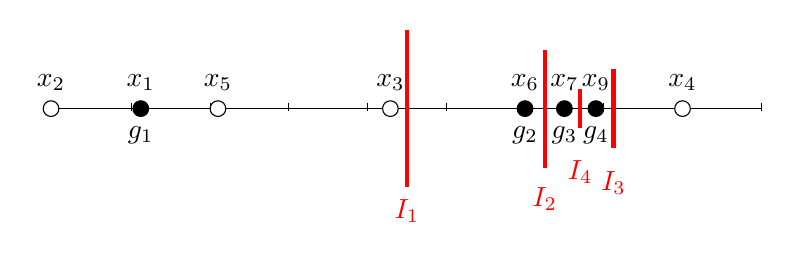
\begin{tikzpicture}
\draw (1,0) -- (10,0);
\foreach \x  in {1,...,10}
  \draw[xshift=\x cm] (0pt,2pt) -- (0pt,-1pt);
% the labels
\node[fill=black,draw=black,circle,inner sep=2pt,label=above:{$x_1$},label=below:{$g_1$}] at (2.12,0) {};
\node[fill=white,draw=black,circle,inner sep=2pt,label=above:{$x_2$}] at (0.98,0) {};
\node[fill=white,draw=black,circle,inner sep=2pt,label=above:{$x_3$}] at (5.29,0) {};
\node[fill=white,draw=black,circle,inner sep=2pt,label=above:{$x_4$}] at (9,0) {};
\node[fill=white,draw=black,circle,inner sep=2pt,label=above:{$x_5$}] at (3.1,0) {};
\node[fill=black,draw=black,circle,inner sep=2pt,label=above:{$x_6$},label=below:{$g_2$}] at (7,0) {};
\node[fill=black,draw=black,circle,inner sep=2pt,label=above:{$x_7$},label=below:{$g_3$}] at (7.5,0) {};
\node[fill=black,draw=black,circle,inner sep=2pt,label=above:{$x_9$},label=below:{$g_4$}] at (7.9,0) {};
\draw[draw=red,ultra thick] (5.5,-1) -- (5.5,1);
\node[text=red] at (5.5,-1.3) {$I_1$};

\draw[draw=red,ultra thick] (7.25,-0.75) -- (7.25,0.75);
\node[text=red] at (7.25,-1.15) {$I_2$};

\draw[draw=red,ultra thick] (8.125,-0.5) -- (8.125,0.5);
\node[text=red] at (8.125,-0.95) {$I_3$};

\draw[draw=red,ultra thick] (7.7,-0.25) -- (7.7,0.25);
\node[text=red] at (7.7,-0.8) {$I_4$};
\end{tikzpicture}
\end{center}

Nuestra subsucesión $\{g_x\}$ es igualmente infinita. Tal y como la hemos definido, tenemos que cada $g_i$ está en un intervalo $(I_i, I_{i-1})$ que cada vez se hace más pequeño. Es decir, que la subsucesión $\{g_x\}$ es de Cauchy y, por lo tanto convergente.

Ahora sólo queda ver cómo podríamos obtener esa subsucesión cuando estamos en espacios que no sean $\real^N$. La idea es sencilla: primero, buscamos una subsucesión que converga en la primera coordenada. Dentro de esa subsucesión, buscamos otra subsucesión que converga además en la segunda, y así con las $N$ coordenadas. 
\end{proof}

\begin{theorem} Sea $K\subset \real$ un conjunto compacto. Entonces, $\appl{f}{\real}{\real}$ es continua en $K$ si existen  $x_m,x_M \in K \tq F(x_m) \leq F(x) \leq F(X_M)\;\forall x \in K$.

Es decir, $F$ es continua en $K$ si alcanza su máximo y su mínimo en el conjunto.
\end{theorem}

\begin{proof}
 Primero, vamos a \textbf{demostrar que el conjunto está acotado superiormente}. Por reducción al absurdo, se puede encontrar una subsucesión convergente que por ser compacto tiene que ser convergente a un elemento pertenciente al conjunto, pero esa sucesión por ser no acotada tenemos: $\exists \gx_n \in K \tq F(\gx_n) \ge n$
 
 Paso 1.2) De manera totalmente análoga.
 
 Paso 2) Vamos a demostrar la existencia de $X_M$:
 Por ser un conjunto acotado, tenemos un supremo en ese conjunto. ¿Ese supremo pertenecerá al conjunto?. Si no perteneciera, podríamos encontrar una subsucesión convergente al supremo lo que contradice la condición de acotado.
 
 \textit{WTF.}
\end{proof}

\paragraph{Aplicación:}
$F(\gor{x}) = |||\gor{x}|||$ una norma (que ya sabemos que es continua):

\emph{Conclusión:} $m \md{x} \leq |||\gor{x}||| \leq C||\gor{x}||$

\begin{theorem}
En $\real^N$ TODAS las normas son equivalentes. 
\end{theorem}

\subsection{Conexión}
\begin{defn}[Conexión\IS por caminos]
Dados $a,b \in C$ podemos encontrar una aplicación continua $\appl{\varphi}{[0,1]}{\real^N}$ tal que $\varphi(0) = a$ y  $\varphi(1) = b$ con $ \varphi(t) \in C\, \forall t \in [0,1]$. 

Es decir, $C$ es conexo por caminos si podemos encontrar una "línea", un camino que una dos puntos cualquiera del conjunto y que además no se salga del conjunto.
\end{defn}

\begin{defn}[Conexión\IS por abiertos]
$C$ es conexo por conjuntos si para cualquier par de abiertos $A,B \subset \real^N \tq C\subset A\cup B$ se cumple que, si $A\cap C\neq \emptyset \y B\cap C \neq \emptyset $ entonces $ A\cap B \neq \emptyset$.

Esto es equivalente a decir que $C$ no puede ser expresado como unión de dos conjuntos disjuntos.
\end{defn}

\begin{remark}
\easyimg{Peine.jpg}{Conjunto \textit{peine}}{imgPeine}

Es curioso comprobar que estas 2 definiciones no son equivalentes. Si tomamos el conjunto peine (figura \ref{imgPeine})
\[ \{(x,0), x\in (0,1]\} \bigcup \{(0,y), y \in (0,1]\} \bigcup \{\displaystyle\bigcup_{n=1}^{\infty}{\left(\frac{1}{n},y\right), y \in [0,1]}\} \]
Podemos razonar que sí es conexo por caminos, pero no según la otra definición.
\end{remark}
\section{Funciones continuas, abiertos y cerrados}
Sea $F$ continua:

1) A abierto $\nimplies F(A)$ abierto.

2) B cerrado $\nimplies F(B)$ cerrado.

\[\appl{F}{\real^N}{\real^N}\]


Definimos
$$F^{-1} (A) = \{\gor{x}\in \real^N \tq F(\gor{x})\in A\}$$
\begin{theorem}[Función inversa]
\begin{itemize}
\item F continua $\y$ A abierto $\implies F^{-1} (A)$ abierto.
\item F continua $\y$ B cerrado $\implies F^{-1} (A)$ cerrado.
\end{itemize}
\end{theorem}

\app
$$M=\{(x,y,z) \in \real^3 \tq x^2 + cos(x|y|) - e^z < 1 \}$$
$$F(x,y,z) = x^2 + cos(x|y|) - e^z < 1 $$
\[M=\{(x,y,z) \in \real^3\}\]
COMPLETAR

\begin{proof}
1)

\[\gor{x} \in F^{-1} (A) \text {Queremos hallar } R>0 \tq B_R(\gor{x})\subset F^{-1} (A)\]
\[\gor{x}\in F^{-1} (A) \dimplies F(\gor{x})\in A\]
\[\exists \varepsilon>0 \tq B_{\varepsilon}(F(\gor{x}))\subset A\]
\[\text{es decir: si} ||\gor{z}-F(\gor{x})|| < \varepsilon \implies \gor{z}\in A\]
\[\text{F continua} \implies \exists \delta > 0 \tq \underbrace{||\gor{x}-\gor{s}||<\delta}_{\gor{s}\in B_R?(\gor{x})} \implies\]
\[\implies ||F(\gor{x})-F(\gor{s})||<\varepsilon. \text{en particular,} F(\gor{s}) \in A; s \in F^{-1} (A)\]
Conclusión: Hemos encontrado un $\delta > 0$ tal que $s \in B_R(\gor{x}) \implies s \in F^{-1} (A)$.
\end{proof}
\subsection{Aplicaciones lineales}
Sea: $\appl{L}{\real^N}{\real^M}$

$L$ es lineal $\dimplies L(\lambda \gor{x}) = \lambda L(\gor{x}) \y L(\gor{x}+\gor{y}) = L(\gx)+L(\gy)$

Además, toda aplicación lineal se puede escribir en forma de matriz.

\[L(\gor{x})=A\gor{x} =
\begin{pmatrix}
a_{11} 	& \cdots & a_{1n}		\\
\vdots	& \ddots &  \vdots 	\\
a_{n1}	& \cdots & a_{nn} 
\end{pmatrix}\]

\begin{theorem}
 L lineal $\implies$ L continua.
\end{theorem}
\begin{proof}
 $$L(\gor{x} = \left(
 \begin{matrix}
  A_1 & \rightarrow \\
  \vdots & \vdots\\
  A_n & \rightarrow
 \end{matrix}\right)$$
 
 COMPLETAR

\end{proof}
\subsection{Norma de matrices}
$$\appl{F}{\real^N}{\real}$$
$$\gor{x} \rightarrow F(\gx) = \underbrace{||A\gx||}_{L(\gx)}$$
F es continua.

Sabemos que existe $c>0$ tal que $||A\gx|| \leq C||\gx||$, es decir,  $||A\gx||\leq C$ si $||\gx||=1$.
$$M = \{||A\gx|| \tq ||\gx||=1\}\subset \real$$\footnote{Conjunto esfera unidad}
La mejor constante $C$ es la cota superior mínima (supremo) que vamos a llamar $\alpha$.\\
$\alpha \in^{?} M$\\
$\alpha$ se alcanza en M, porque F es continua y M es compacto.


\begin{defn}[Norma de una matriz]
$$|||A||| = \alpha = max{||A\gx||\tq||\gx||=1}$$
Ejercicio propuesto: demostrar que $|||\cdot|||$ es una norma.
\end{defn}
Demostración de la 4' porpiedad:
$$|||A+B||| = max{||(A+B)\gx|||} = ||(A+B)\gx_{A,B}|| = ||A\gx_{AB} + B\gx_{AB}|| \leq$$
$$
\underbrace{||A\gx_{AB}||}_{\leq max||A\gx|| =
|||A|||} + \underbrace{||B\gx_{AB}||}_{|||B|||} $$

\paragraph{Ejemplo:}COMPLETAR
Sea $A = \begin{pmatrix}
      1&2\\-3&1\\3&0
     \end{pmatrix}$. Calcular su norma.
Resolución:
Acabamos teniendo que maximizar (sabiendo que $|x|+|y| = 1$: $|x+2y| + |-3x+y| + |2x| \leq |x|+|2y| + |3x| + |y| + 2|x| = 6|x|+3|y| \leq 6 (|x|+|y|) =6$
¿Podemos encontrar un vector $(x_0,y_0)$ tal que $||A(x_0,y_0)^T||_1 = 6$?\\
Tomando $x_0 = 1$ y $y_0 = 0$ lo encontramos.
\obs Coincide con la suma de los valores absolutos de las columnas y escoger el más grande.

Aplicando lo mismo con la norma infinito: COMPLETAR
COMPLETAR

\begin{lemma}
 Sea A una matriz, $A^TA$ es simétrica.
\end{lemma}
\begin{lemma}
 $\underbrace{<\gx,A\gy>}_{\text{Producto en } \real^n} = \underbrace{<A^T\gx,\gy>}_{\text{Producto en } \real^M}$
\end{lemma}

 $A^TA$ diagonalizable ($N \times N$). Dado $\gx \in \real^N$.

 Desarrollamos en $B$: $\gx = \sum \alpha_i \gor{v}_i$. Con $<v_i,v_j> = 0$ con $i \neq j$.

 Calculamos $||\gx|| = \sum \alpha_i^2<v_i,v_i>$
 
 $$A^TA\gx = (A^TA)(\sum \alpha_i v_i) = \sum (\alpha_i\lambda_i\gor{v_i})$$
 
 Queremos hallar el máximo de $||A\gx||$ cuando $||\gx|| = 1$.
 
 $$||A\gx||^2 = <A\gx,A\gx> = <A^TA\gx,\gx> = \underbrace{<\sum \lambda_i \alpha_i v_i,\sum\alpha_i v_i>}_{<v_i,v_j> =0 \text{ con } i \neq j.}$$
 $$= \sum \lambda_i \alpha_i^2 \leq \lambda_{max} (\sum \alpha_i^2) = \lambda_{max}$$
 
 \paragraph{Conclusión: }
 Hemos demostrado que:
 $$ max||A\gx|| \underbrace{\leq}_{=} ({\lambda_{max}})^{\frac{1}{2}}$$
 Este máximo se puede alcanzar tomando $x$ como el autovector asociado, por lo que el $\leq$ se convierte en un $=$.
 
 \section{Limite}
 $\appl{F}{\real^N}{\real^M}$
 \begin{defn}[Límite]
  $$\lim_{\gx \rightarrow \ga} F(\gx) = \gor{L} \dimplies \forall \varepsilon > 0,  \exists \delta>0 \tlq 0<||\gx-\ga|| <\delta \implies ||F(\gx) - L||<\varepsilon$$
 \end{defn}
 Importante el detalle de $0 < ||\gx-\ga||$, no es un $\leq$, porque no se necesita que la función esté si quiera definida en el punto $\ga$.  
 
 \begin{theorem}
  
  Sean $\gor{x_n} = (x_1,...,x_n) \in \real^N$ y $\gor{L} = (L_1,...,L_n) \in \real^N$.
 
  $$x_n \rightarrow \gor{L} \dimplies (x_1 \rightarrow L_1) \y (x_2 \rightarrow L_2) \y ... \y (x_n \rightarrow L_n)$$
 \end{theorem}
 
 Idea para el cálculo de límites: 
 \begin{itemize}
  \item $\displaystyle\mylim{x}{a}{x} = \lim_{\gy\rightarrow 0} F(\gy+\ga)$.
  \item Límite a lo largo de rectas. $\displaystyle\mylim{x}{a}{\gx} \sim \lim F({t\gor{v}})$
 
 \end{itemize}
 
 Si $\displaystyle\lim F({t\gor{v}})$ toma valores distintos dependiendo de $\gor{v} \dimplies \nexists \displaystyle\mylim{x}{0}{\gx}$
 
 Pero, si $\forall t \in \real, \mylim{x}{a}{t\gor{v}} = L \implies \gor{L}$ es el candidato a ser el límite (no tiene porque serlo). El siguiente paso sería demostrar con argumentos de comparación (Sandwich) u otros que $\mylim{x}{a}{\gx} = L$.
 
 El contraejemplo es $f(x,y) = \frac{x\cdot y^2}{x^2 + y^4}$. Veamos por que:
 
 Nos acercamos al límite por medio de rectas:
 $$f(x,y) = f(x,mx) = \frac{x\cdot(mx)^2}{x^2 + (mx)^4} = \frac{m^2x^3}{(1 + x^2m^4)x^2}.$$
 $$\displaystyle\lim_{x\rightarrow 0} (f(x,mx)) \rightarrow 0, \forall m \in \real$$
 Pero si nos acercamos al límite por medio de $x = y^2$ tenemos:
 $$f(x,y) = f(y^2,y) = \frac{y^2y^2}{y^4+y^4} = \frac{y^4}{2y^4} = \frac{1}{2}\neq 0$$
 \paragraph{Conclusión:}
 
 $$\lim_{(x,y) \rightarrow (0,0)} (f(x,y)) \neq 0$$
 
 
\begin{theorem}
 $F$ continua $\dimplies$ para cualquier abierto $A$, $F^{-1}(A)$ es abierto.
\end{theorem}
\obs
Si $\appl{F}{\omega\subset\real^N}{\real^M} \dimplies$ para cualquier abierto $A, F^{-1}(A) = \omega \cup V$, con $V$ abierto.

\begin{proof}
$\implies$ De este teorema ya teníamos demostrada la implicación $\implies$.

$\Leftarrow$ Queremos probar: $$\forall \varepsilon > 0, \exists \delta>0 \tlq ||\gx-\ga||<\delta \implies \underbrace{||F(\gx)-F(\ga)||<\delta}_{F(\gx)\in B_{\varepsilon}(F(\ga))}$$
Tomamos  $$A = B_{\varepsilon}(F(\ga)) \rightarrow F(\ga) \in A \implies \ga \in F^{-1}(A)$$
Por hipótesis, $F^{-1}(A)$ abierto $\y$ $\ga \in F^{-1}(A)$
$$\exists B_{\delta}(\ga) \subset F^{-1}(A) \text{.Es decir, } \gor{s}\in B_{\delta}(\ga) \subset F^{-1}(A), s\in F^{-1}(A) \implies F(s) \in A = B_{\varepsilon}(F(\ga))$$

\end{proof}
\begin{remark}
Este teorema también se cumple para cerrados.
\end{remark}
\section{Diferenciación}

\begin{defn}
 $F$ diferenciable en $\gor{a}$ si 
 
 $$\exists \text{ aplicación lineal L} \tlq \frac{F(\gx)-F(\ga)-L(\gx-ga)}{||\gx-\ga||} \underbrace{\rightarrow}_{\gx\rightarrow\ga} 0$$
$$ = \lim_{\gor{h} \rightarrow \ga} \frac{\md{F(\ga+\gor{h}) - F(\ga) - L\gor{h}}}{||\gor{h}||}$$

\end{defn}


\obs
\begin{itemize}
\item Si existe, $L$ es única.
\end{itemize}

\begin{proof}
Supongamos que existen $L_1,L_2$.
\[0=\lim_{\gor{h} \rightarrow \gor{0}} \frac{F(\gor{a}+\gor{h}) - F(\ga)-L_1\gor{h}}{||\gor{h}||} = \lim_{\gor{h} \rightarrow \gor{0}} \frac{F(\gor{a}+\gor{h}) - F(\ga)-L_2\gor{h}}{||\gor{h}||}\].

$$\text{ Sumando: } 0 = \lim_{\gor{h} \rightarrow \gor{0}} \frac{||F(\gor{a}+\gor{h}) - F(\ga)-L_1\gor{h}|| + ||F(\gor{a}+\gor{h}) - F(\ga) -L_2\gor{h}||}{||\gor{h}||}$$

\obs $||A-B|| = ||A+(-B)|| \leq ||A||+||B||$

$$\leq \lim_{\gor{h} \rightarrow \gor{0}} \frac{2\cdot\md{F(\ga + \gor{h}) - F(\ga)} + \md{L_1\gor{h}} + \md{L_2\gor{h}}}{\md{\gor{h}}}$$

Completar la contradicción.
\end{proof}

\paragraph{Notación: (Diferencia de $F$ en $\ga$)}

$$L\equiv DF(\ga)$$ 

\paragraph{Proposición:}
$$F \text{ diferenciable en } \ga \implies F \text{ continua en } \ga$$
\begin{proof}
 $$\lim_{\gor{h} \rightarrow \gor{0}} \frac{||F(\ga+\gor{h}) - F(\ga) - L\gor{h}}{||\gor{h}||} = 0$$
 Esta es la definición de diferenciable. Para que este límite sea 0, el numerador tiene que tender a 0, por lo que $F(\ga+\gor{h}) - F(\ga) \rightarrow 0$
\end{proof}

\obs
$F$ diferenciable en $\ga$.
\begin{align*}
\appl{F}{\real^N}{\real^M}\\
\text{Sabemos:}\\
 0 = \lim_{\gor{h} \rightarrow \gor{0}} \frac{||F(\ga+\gor{h}) - F(\ga) - L\gor{h}}{||\gor{h}||} = 0 \\
 \text{En particular (tomando } h = t \gor{e_1})\\
 \lim_{\gor{t} \rightarrow \gor{0}}\frac{a}{b} = \lim_{\gor{t} \rightarrow \gor{0}}\norm{\underbrace{\frac{1}{t} F(\ga+t\gor{e_1})-F(\ga))-L\gor{e_1}}_{\gor{W}(t)\in\real^N}}\\
 \text{Tomando la componente k-esima}\\
 0 = \mylim{t}{0}{\frac{F_K(a+te_i)-F_k(a)}{t} - L_{ki}}\\
 L_{ki} = \mylim{t}{0} {\frac{F_k(a+te_i) - F_k(a)}{t}} = \deriv{ F_k}{x_i}(\ga)
\end{align*}

\paragraph{Nomenclatura: }
Aproximación lineal $\sim$ Diferencial.

Matriz jacobiana $\sim$ Jacobiana.

\begin{theorem}
 Matriz asociada a $DF(\ga) \equiv $ Matriz de las derivadas parciales de F.
 
 $$DF(\ga) \equiv \begin{pmatrix}
                \dpa{F_1}{x_1} & \cdot & \dpa{F_1}{x_N}\\
                \vdots& \ddots & \vdots\\
                \dpa{F_N}{x_1} & \cdot & \dpa{F_N}{x_N}
                \end{pmatrix}
$$
\end{theorem}

\begin{theorem}
 $F$ diferencialbe en $\ga \implies \exists \deriv{F_k}{x_i}(\ga), i=1,2,...,N \y k = 1,2,...,M$
\end{theorem}

El contraejemplo para demostrar $\Leftarrow$ es el mismo que en los límites a lo largo de rectas.

$f(x,y) = \left\{ \begin{matrix}

\frac{xy^2}{x+y^2} & (x,y) = (0,0) \\ 
0 & (x,y)=(0,0)
           
          \end{matrix}\right.
$
\paragraph{Comentarios sobre notación: }
\begin{itemize}
 \item $\appl{\delta}{\real}{\real^M}$. Utilizamos notación vectorial en vez de matricial (porque tendríamos una matriz columna).\\
 Ejemplo: la velocidad (en un instante de tiempo, un punto en el espacio).
 \item $\appl{F}{\real^N}{\real}$ (función escalar):

 COMPLETAR
 Se suele llamar vector gradiente.
 \item 
\end{itemize}

\subsection{Regla de la cadena: }
\paragraph{Derivada de una composición:\\}

COMPLETAR DIBUJITO

$\appl{F}{\real^N}{\real^M}$. 

$\appl{G}{\real^M}{\real^K}$.

$\appl{H=G\circ F}{\real^N}{\real^K}$.

$ \gx \in \real^N, \gy \in \real^M$

$F$ diferenciable en $\ga$, $G$ diferenciable en $F(\gor{a})$. Entonces $H=G\circ F$ es diferenciable en $\ga $.
Además la expresión matricial es:

$\underbrace{DH(\ga)}_{K\times N} = \underbrace{DG(F(\ga))}_{K\times M}\cdot \underbrace{DF(\ga)}_{M\times N}$
 
\obs
\paragraph{Notación de Leibniz:}

Para calcular 1 único elemento de la matriz diferencial (el de la fila $i$, columna $j$):

$$\deriv{H_i}{x_j}(\ga) = \displaystyle\sum_{k=1}^M \deriv{G_i}{y_k}\cdot\deriv{F_k}{x_j}$$
Con cuidado de $\displaystyle \deriv{G_i}{y_k}$ evaluado en $\displaystyle F(\ga)$ y $\displaystyle\deriv{F_k}{x_j}$ evaluado en $\ga$.

\paragraph{Aplicaciones y ejemplos:}
\begin{itemize}
 \item 
 $\appl{F}{\real^N}{\real}$
 
 $\appl{\sigma}{\real}{\real^N}$
 
 Sea $g\equiv F\circ \sigma \equiv \text{ Comportamiento de F a lo largo de la curva } \sigma, \appl{g}{\real}{\real}$.

$$g'(t_0) = DF(\sigma(t_0))D\sigma(t_0) = \underbrace{...}_{\text{Notación matricial}} = \underbrace{\pesc{\nabla F(\sigma(t_0))}{\sigma'(t_0)}}_{\text{Notación vectorial}}$$

 
 \item 
 $\sigma(t) = t\gor{b} + (1-t)\ga$
 
 $\appl{F}{\real^N}{\real^M}$
 
 $F\circ \sigma(t) \equiv g(t)$
 
 COMPLETAR
\end{itemize}

\subsection{Extensiones del teorema del Valor Medio}
\begin{itemize}
 \item Original:
 $\appl{f}{\real}{\real}$ diferenciable. 
 
 $f(b)-f(a) = f'(c)(b-a)$ para algún $c\in[a,b]$
 
 \item
  
 $F : \real^N  \longrightarrow \real$
 
 $\sigma(t)  = t(\gor{b})+(1-t)\gor{a}$
 
 $g  = F\circ \sigma$
 $\appl{g}{\real }{\real}$
 
 $F(\gor{b}-\gor{a}) = g(1)-g(0)  = g'(s) \text{ para algún }s\in[0,1]$
 
  
  Peeeeero...
  $$\appl{F}{\real^N}{\real^2}$$
  $$F(\gor{b})-F(\ga) = \begin{pmatrix}
                         \pesc{\nabla F_1(\gor{c_1}),{\gor{b}-\ga}}\\
                         \pesc{\nabla F_2(\gor{c_2}),\gor{b}-\ga}
                        \end{pmatrix}
$$
  Tenemos 2 $c$ distintos, uno para cada $f$, por lo que este teorema pierde sentido.
  
  \item Versión para funciones matriciales:
  
  \begin{theorem} [Extensión del valor medio]
  Sea $f \in C^1$ en un abierto que contenga $[a,b]$.
  $$\norm{F(\gor{b}-\ga)} \leq |||DF(\gor{c})|||\cdot\norm{\gor{b}-\ga}$$ 
  
  Siendo c un punto del segmento que une $\ga$ y $\gb$ en el que $|||DF(tb+(1-t)a)|||$ alcanza su máximo.
   
  \end{theorem}

  
  
  \begin{proof}
   i) $$\appl{f}{\real}{\real}$$
   $$f(\gor{b}-f(\ga) = g(1)-g(0) = \int_0^1g'(s)ds \text{ con } g(t) = f(tb+(1-t)a)$$
   
   ii)  $$\appl{h}{\real^N}{\real}$$
   $$h(\gor{b}-h(\ga) = g(1)-g(0) = \int_0^1g'(s)ds = \int_0^1 \pesc{\nabla h(s\ga+(1-s)\gor{b}),(\gor{b}-\ga)}$$
   $$g(t) = h(tb+(1-t)a)$$
   
   iii) $$\gor{G} = (G_1,...,G_M), G_i = \int_0^1H_i(t)dt$$
   Con $\gor{H} = (H_1(t),...,H_M(t))$
   
   
   $$\norm{\gor{G}}^2 = \pesc{\gor{G},\gor{G}} = \sum_{i=1}^M \left(\int_0^1 H_i(t)dt\right) \underbrace{\left(\int_0^1 H_i(s)ds\right)}_{G_i}$$
 
   $$\norm{\gor{G}}^2 = \displaystyle\int_0^1 \left(\underbrace{\sum_{i=1}^M G_i H_i (t)}_{\pesc{\gor{G},\gor{H}(t)}\leq \norm{\gor{G}}\cdot \norm{\gor{H}}}\right)dt$$
   Conclusión:
   $$\norm{\gor{G}}^2 \leq \displaystyle\int_0^1\norm{G}\cdot\norm{H(t)}dt$$
   
   iv) $\appl{F}{\real^N}{\real^M}$
   
   $\appl{F_i}{\real^N}{\real}$
   
   $\underbrace{F_i(\gor{b})-F_i(\ga)}_{G_i} = \displaystyle\int_0^1 \underbrace{\pesc{\nabla F_i (s\gor{b}+(1-s)\ga ),(\gor{b}-\ga)}}_{H_i(t)}dt$
   
   Por el apartado iii tenemos que:
   
   
   $$\gor{H}(t) = \begin{pmatrix}
                   H_1(t)\\
                   \vdots\\
                   H_M(t)
                  \end{pmatrix}
                = \begin{pmatrix}
                   \pesc{\nabla F_1(tb+(1-t)a),b-a}\\
                   \vdots\\
                   \pesc{\nabla F_M(tb+(1-t)a),b-a}
                  \end{pmatrix}
		= \left(DF(...)\right)\begin{pmatrix}
		                        b_1-a_1\\
		                        \vdots\\
		                        b_M-a_M
		                       \end{pmatrix}
$$

$$\norm{H(t)} = \norm{DF(...)(\gor{b}-\ga)} \leq \norm{DF}\cdot\norm{\gor{b}-\ga}$$


$$\norm{F(\gor{b})-F(\ga)} \leq \displaystyle\int_0^1 \norm{\nabla DF_i(tb+(1-t)a),b-a}dt$$

Aplicando: $A\gor{v} \leq |||A|||\cdot \norm{\gor{v}}$

$$\norm{F(\gor{b})-F(\ga)} \leq \displaystyle\int_0^1 |||DF(*)|||\cdot\norm{\gb-\ga}dt$$
$$= \norm{\gb - \ga} \displaystyle \int_0^1 |||DF(tb+(1-t)a)||| dt \leq |||DF(\gor{c})|||\cdot\norm{\gb-\ga}$$ 

Siendo c un punto del segmento que une $\ga$ y $\gb$ en el que $|||DF(tb+(1-t)a)|||$ alcanza su máximo.
   
Conclusión:

$$\norm{F(\gor{b})-F(\ga)} \leq \norm{DF}\cdot\norm{\gor{b}-\ga}$$
  \end{proof}

\end{itemize}

\paragraph{Aplicación:\\}

$\appl{F}{\real^N}{\real^M}, F \in C^1$, definida en un conjunto abierto y conexo.

$DF(\gx) \equiv 0, \forall \implies F \equiv $ cte.	

\subsection{Derivada direccional: }

$\appl{F}{\real^N}{\real^M}$ (escalar)

$\ga \sim$ Recta que pasa por $\ga$ con dirección $\gor{v}$.

$r(t) = \ga + t\gor{v}$. 

\obs
Como una recta tiene infinitos vectores directores (dependiendo de la longitud), siempre tomaremos vectores directores unitarios, con $\norm{\gor{v}} = 1$.


Vamos a estudiar: $g(t) = F(\ga + t\gor{v}) = F \circ r (t)$.

$t \sim 0 \dimplies \ga + t\gor{v} \sim \ga$
\begin{defn} [Regla de la cadena]
$$g'(0) = \displaystyle\lim_{h \rightarrow 0} \frac{g(h)-g(0)}{h} = \displaystyle\lim_{h \rightarrow 0} \frac{F(\ga+h\gor{v})-F(\ga)}{h} \equiv D_{\gor{v}}F(\ga)$$. 
\end{defn}

\obs
La existencia de $D_{\gor{v}}F(\ga), \forall \gor{v}\in \real^N$ NO garantiza que $F$ sea derivable.


Si sabemos que $F$ SÍ es diferenciable podemos usar la regla de la cadena obteniendo:

$D_{\gor{v}}F(\ga) = g'(0) = D(F\circ r)(0) = ... = \pesc{\nabla F(\ga),\gor{v}}$


\paragraph{Aplicación:} 
\begin{itemize}
 \item 
 Dirección de máximo crecimiento:

$D_{\gor{v}}F(\ga) = \pesc{\nabla F(\ga),\gor{v}}\leq \norm{\nabla F(\ga)}\cdot \underbrace{\norm{\gor{v}}}_{\equiv 1}$

Conclusión:
\begin{align*}
D_{\gor{v}}F(\ga) &\leq \norm{\nabla F(\ga)}\\
&\uparrow\\
\text{El }= \text{se obtien}&\text{e cuando }\gor{v} = \displaystyle \frac{\nabla F(\ga)}{\norm{\nabla F(\ga)}}. 
\end{align*}

 
 \item
 Vector perpendicular a los conjuntos de nivel
 
 $\appl{F}{\real^N}{\real^M}$
 
 $S = \{ \gx \in \real^N \tq F(\gx) = 0\}$ (Conjunto de nivel)
 
 $\ga \in S$
 
 Entonces: $\nabla F(\ga) \perp S$
\end{itemize}

\begin{theorem}[Derivadas parciales continuas implican función diferenciable]
Si existen todas las derivadas parciales y son continuas $\implies F$ diferenciable en $\ga$.
 
\end{theorem}

Contraejemplo de la no reciprocidad: $f(x) = x^2 sin\left(\frac{1}{x}\right)$

\begin{proof}
 $\appl{F}{\real^2}{\real}$
 
 $$¿\frac{\left|F(a+a,b+k) - F(a,b) - \deriv{F}{x}(a,b) h - \deriv{F}{y}(a,b)k\right|}{\norm{(h,k)}}\longrightarrow 0?$$
 
 Sumamos y restamos al numerador $F(a,b+k)$.
 
 $$\frac{\left|\left(\underbrace{F(a+h,b+k) - F(a,b+k)}_{\deriv{F}{x}(a+\tilde{h},b+k) \text{ para algún } 0 \leq\tilde{h}\leq h} -  \deriv{F}{x}(a,b) h\right) + \left(\underbrace{F(a,b+k) - F(a,b)}_{\deriv{F}{x}(a+h,b+\tilde{k}) \text{ si } 0 \leq\tilde{k}\leq k}- \deriv{F}{y}(a,b) k\right)\right|}{\sqrt{h^2+k^2}}$$

 $$0\leq\frac{\left|\deriv{F}{x}(a+\tilde{h},b+k)-\deriv{F}{x}(a,b)\right| \cdot |h| + \left| \deriv{F}{y}(a,b+\tilde{k}) - \deriv{F}{y}(a,b)\right| \cdot |k|}{\sqrt{h^2+k^2}} = (*)$$
 
 Aquí es donde aplicamos que las derivadas parciales son continuas: como $h$ y $k$ son pequeños (por lo tanto $\tilde{h}<h$ también lo será) los puntos $(a,b)$ y $(a+h,b+k)$ también están cerca, por lo que sus imágenes por la derivada estarán también cerca, es decir, $|\deriv{F}{x}(a,b)-\deriv{F}{x}(a+\tilde{h},b+k)| \rightarrow 0$ y lo mismo con la otra.
 
 Conclusión:
 
 \begin{align*}
0 \leq (*) \leq \varepsilon \frac{|h|+|k|}{\sqrt{h^2+k^2}} &\leq C\varepsilon \rightarrow 0 \text{ cuando } \gor{h},\gor{k} \rightarrow \gor{0}\\
&\uparrow\\
\text{El numerdador es la} & \text{ norma 1 y el denominador la norma 2.}\\
\text{En } \real^N &\text{ todas las normas son equivalentes.}  
 \end{align*}
 
 
\end{proof}


\subsection{Derivadas iteradas:}

\paragraph{Notación:}

$\deriv{}{y}\left(\deriv{f}{x}\right) \equiv \deriv{^2f}{x \partial y}$

\begin{theorem}[Euler (orden de las derivadas)]
Si las derivadas segundas son continuas, entonces:
$$\deriv{^2f}{x_i\partial x_j} = \deriv{^2 f}{x_j \partial x_i}$$
\end{theorem}

\subsection{Máximos y mínimos}

\index{Máximo/mínimo!local}
\begin{defn}[Máximo/mínimo local] Sea $\appl{f}{\real^N}{\real}$. Diremos que $\vx_0 \in \real^N$ es un punto de máximo local si $\exists \epsilon > 0 \tq F(\vx_0) \geq F(\vx)\;\; \forall \vx \in B_{\epsilon} (\vx_0) $

La definición es análoga para el mínimo\end{defn}

\begin{remark} Por las propiedades del gradiente, si $F$ es diferenciable y $\vx_0$ es un máximo o mínimo local, entonces debe ser $\nabla F(\vx_0) = \vec{0}$.\end{remark}

\index{Punto!crítico}
\begin{defn}[Punto crítico] $\vx \in \real^N$ es un punto crítico de $F$ si y sólo si $\nabla F(\vy) = \vec{0}$\end{defn}

No todos los puntos críticos son máximos o mínimos, así que tenemos que clasificarlos de alguna forma. Para ello, usamos el polinomio de Taylor de orden 2, de forma que 

\[F(x,y) = F(x_0, y_0) + \pesc{\nabla F(x_0, y_0), (x-x_0, y-y_0)} +\]\[\frac{1}{2}(x-x_0, y-y_0)\left(\begin{matrix} \frac{\partial^2 f}{∂ x^2} (x_0,y_0) & \frac{\partial^2 f}{\partial x \partial y} (x_0,y_0) 
\\ \frac{\partial^2 f}{\partial y \partial x} (x_0,y_0) & \frac{\partial^2 f}{\partial y^2} (x_0,y_0) \end{matrix}\right) \left(\begin{matrix} x - x_0 \\ y - y_0 \end{matrix}\right) + \epsilon \]

Simplificando nos queda que:

\[F(\vx) = F(\vx_0) + \pesc{\nabla F(\vx_0),\vx - \vx_0} + \frac{1}{2}(\vx - \vx_0) D^2F(\vx_0) (\vx - \vx_o) ^T + \epsilon\]

Dado que el gradiente es 0, el punto clave es el signo de $\frac{1}{2}(\vx - \vx_0) D^2F(\vx_0) (\vx - \vx_o) ^T$. Para ello, usamos las siguientes definiciones del álgebra lineal.

\subsubsection{Resultados de álgebra lineal}
\index{Matriz!semidefinida positiva/negativa}
\index{Matriz!definida positiva/negativa}
\begin{defn}[Matriz semidefinida y definida positiva y negativa]\noindent\\ \indent
La matriz $A$ de dimensión $N\x N$ es semidefinida positiva si y sólo si $\vv A \vv^T \geq 0 \;\; \forall \vv \in \real^N$.

La matriz $A$ de dimensión $N\x N$ es definida positiva si y sólo si $\vv A \vv^T > 0 \;\; \forall \vv ≠0 \in \real^N$.

La matriz $A$ de dimensión $N\x N$ es semidefinida negativa si y sólo si $\vv A \vv^T \leq 0 \;\; \forall \vv \in \real^N$.

La matriz $A$ de dimensión $N\x N$ es definida negativa si y sólo si $\vv A \vv^T < 0 \;\; \forall \vv ≠0 \in \real^N$.
\end{defn}

\begin{theorem}
Si una matriz es simétrica, existe una base en la cual la matriz es diagonal.
\end{theorem}

\index{Autovalor}
\index{Autovector}
Sea $A$ una matriz $N\x N$. Entonces diremos que un vector $\vv ≠ \vec{0}$ es un autovector asociado al autovalor $\lambda\in \real$ si y sólo si $A\vv = \lambda\vv$. Dado que podemos escribir

\[ A = \left(\begin{matrix}
a & b \\ c &  d
\end{matrix}\right)\;\;\;\; \vv = \left(\begin{matrix}
x\\ y
\end{matrix}\right) \], entonces tenemos que $A\vv = \lambda \vv$ si y sólo si

\[ \left\lbrace\begin{matrix}ax+by=\lambda x \\ cx+dy = \lambda y \end{matrix}\right. \]

Es decir, la autorrecta $\begin{pmatrix} x \\ y \end{pmatrix}$ es una solución no trivial del sistema anterior. Sin embargo, para que haya soluciones no triviales el determinante de la matriz $\begin{pmatrix}a-\lambda & b \\ c & d - \lambda\end{pmatrix}$ debe ser 0.

Por lo tanto, los autovalores son las soluciones de la ecuación $det(A-\lambda I) = 0$, siendo $I$ la matriz identidad.

\begin{theorem}
Si un conjunto de autovectores es una base, entonces la matriz $A$ expresada respecto a esa base pasa a ser diagonal, y los elementos de la diagonal son los autovalores. 

Si dos autovalores son distintos, los autovectores asociados son distintos.

Si A es simétrica, entonces el conjunto de autovectores es una base.
\end{theorem}

Volvemos ahora al cálculo.

\begin{theorem}[Clasificación de puntos críticos]
Sea $\appl{F}{\real^N}{\real}$, $F\in C^2$ (con dos derivadas continuas), y sea $\vx_0$ un punto crítico. Entonces

\begin{enumerate}
\index{Máximo/mínimo!local}
\index{Punto!de silla}
\index{Punto!crítico degenerado}

\item Si \textbf{todos} los autovalores de $D^2F(\vx_0)$ son \textbf{mayores que cero}, entonces $D^2F(\vx_0)$ es definida positiva y $\vx_0$ es un \textbf{mínimo local}.
\item Si \textbf{todos} los autovalores de $D^2F(\vx_0)$ son \textbf{menores que cero}, entonces $D^2F(\vx_0)$ es definida negativa y $\vx_0$ es un \textbf{máximo local}.
\item Si \textbf{algunos} autovalores son \textbf{mayores que cero} y otros son \textbf{menores que cero}, entonces $\vx_0$ es un \textbf{punto de silla.}
\item Si algún autovalor \textbf{es 0}, y el resto son mayores o menores que cero, entonces $\vx_0$ es un \textbf{punto crítico degenerado}.
\end{enumerate}
\end{theorem}

\subsubsection{Ejemplos}

Tomamos $F(x,y) = x^2 + y^2 +xy$. Obtenemos los puntos críticos, es decir, los puntos en los que $\nabla F(x,y) = (0,0)$. El punto resultante es $(0,0)$. Estudiamos el tipo de punto crítico. Para ello, calculamos la matriz hessiana en ese punto:

\[ D^2F(0,0) = \begin{pmatrix}2&1\\1&2\end{pmatrix}\]. 

Los autovalores son las soluciones de

\[ 0 = det\left(\begin{pmatrix}2&1\\1&2\end{pmatrix} - \lambda \begin{pmatrix}1&0\\0&1\end{pmatrix}\right) = det\begin{pmatrix}2-\lambda & 1 \\ 1 & 2-\lambda\end{pmatrix} = (2-\lambda)^2  - 1\]

Por lo tanto, $\lambda$ es $3$ o $1$. Dado que ambos autovalores son mayores que 0, entonces $D^2F$ es definida positiva y $(0,0)$ es un mínimo local.

\subsection{Máximos y mínimos absolutos}

\index{Máximo/mínimo!absoluto}
\begin{defn}[Máximo y mínimo absoluto] Sea $\appl{F}{\real^N}{\real}$ y $A\subset \real^N$. $\vx_m$ es un máximo absoluto de $F$ en $A$ si y sólo si $F(\vx_m) ≥ F(\vx)\;\; \forall \vx \in A$. La definición es análoga para el mínimo.
\end{defn}

\begin{theorem}[Teorema de compacidad]
Tenemos un conjunto $K\subset \real^N$ compacto (cerrado y acotado). Supongamos la sucesión $\{\vx_n\}_{n\in\nat}\subset K$. Entonces podemos encontrar al menos una subsucesión $\{\vx_{n_j}\}_{j\in\nat} \subset \{\vx_n\}_{n\in\nat}$ tal que $\{\vx_{n_j}\}$ es convergente.
\end{theorem}

\begin{proof}
Trabajamos en dimensión 2, pero la demostración es análoga.
Como $K$ es compacto, podemos encontrar un cuadrado $Q_0$ de lado $L$ que encierre completamente a $K$. Divido $Q_0$ en $2^2$ cuadrados de lado $L/2$.  En alguno de ellos hay infinitos términos de la sucesión: lo llamamos $Q_1$ y me quedo con uno de los términos de la sucesión, al que llamamos $x_1$. Volvemos a dividir este cuadrado en cuatro cuadrados, elegimos uno que tenga infinitos términos de la sucesión y seleccionamos un elemento de la sucesión dentro al que llamamos $x_2$. Repetimos esto muchas veces, de forma que cada término $x_n$ está encerrado en el cuadrado $Q_n$ de lado $\frac{L}{2^n}$. 

Si $k,l > n$, entonces es claro que $\md{\vx_k-\vx_l}$ es menor o igual que la diagonal de $Q_n$, que es $\frac{L}{2^n}\sqrt{2}$, que tiende a cero cuando $n\to\infty$. Por el criterio de Cauchy, entonces esta sucesión es convergente, y como $K$ es cerrado el límite pertence a $K$.
\end{proof}

\begin{theorem}
Sea $K\subset \real^N$ compacto y $\appl{F}{\real^N}{\real}$, continua en $K$. Entonces, $F$ alcanza su máximo y mínimo absolutos en $K$.
\end{theorem}

\begin{proof}

Como $F$ es acotada, existe $\alpha = \sup \{ F(x) \tq x \in K\}$. Existe entonces una sucesión $\{x_n\}$ tal que si $n\to \infty$ entonces $F(x_n)\to \alpha$. 
Sabemos que existe $\{x_n\}\subset K$, por lo que existe una subsucesión$\{x_{n_j}\}$ convergente tal que $x_{n_j} \to x_0 \in K$

Como $F$ es continua, $F(x_{n_k})\to F(x_0)$, es decir $F(x_{n_j}) \to \alpha$, por lo tanto el supremo es el máximo.
\end{proof}

\subsubsection{Ejemplos}

La función a estudiar es $F(x,y) = x^2-y^2$ en la bola $\omega = \{ x^2 + y ^2 ≥ 1\}$. Es diferenciable en todo $\real$ porque es un poliniomio. 

Calculamos el diferencial y vemos qué ocurre cuando es 0 \[\nabla F = (2x, -2y) = (0,0) \implies (x,y) = (0,0)\]

Operando, vemos que el punto $(0,0)$ es un punto de silla. Ahora sólo queda ver el comportamiento en la frontera $C$, cuando $x^2+y^2 = 1$. $F$ restringida a $C$ quedaría de la siguiente forma:

\[ F(\cos t, \sin t) = \cos^2 t - \sin^2 t = \cos 2t\]

El coseno tiene máximos cuando $t=0$ y $t=\pi$, y mínimos cuando $t=\pi /2$ y $t=3\pi /2$. Es decir, tiene máximos absolutos en los puntos $(1,0),\;(-1,0)$ y mínimos absolutos en $(0, -1)$, $(0, 1)$. 

\index{Multiplicadores de Lagrange}
\begin{theorem}[Multiplicadores de Lagrange]
Tenemos una función $\appl{F}{\real^2}{\real}$ y una restricción $G(x_1,\cdots,x_n) = k$, resolvemos el siguiente sistema:

\begin{align*}
\nabla F &= \lambda \nabla G \\
G &= k
\end{align*} 

\end{theorem}


\subsection{Desarrollo de Taylor}

$\appl{F}{\real^N}{\real}. F\in C^k$\footnote{F es k veces derivable}. 

Queremos desarrolar $F$ alrededor de $\ga \in \real^N$.

Dimensión 1) $g(x) = g(0) + g'(0)x + \frac{g''(0)}{2!}x^2 + ... + \frac{g^{k)}(0)}{k!}x^k + \underbrace{error}_{\frac{g^{k+1)}(s)}{(k+1)!}x^{(k+1)}}$

$F(\ga + \gor{h}) = F(\ga) + ...$

Más dimensiones) 

Tomamos $g(t) \equiv F(t(\ga + \gor{h}) + (1-t)\ga)$. Así hemos reducido el cálculo a dimensión 1.

%\begin{gather}

$$g'(t) = \pesc{\nabla F(a+th),h} = \sum_{i=1}^N \deriv{F}{x_i}(a+th)\cdot h_i$$
$$g'(0) = \pesc{\nabla F(\ga), \gor{h}}$$
$$g''(t) = \sum_{i=1}^N\left(\sum_{j=1}^N \deriv{}{x_j}\deriv{F}{x_i}(\ga+\gor{h})\cdot{h_j}\right)h_i = \sum_{i,j = 1}^N \deriv{^2F}{x_i \partial x_j}(\ga+t\gor{h})h_ih_j $$

Iterando:

$$\frac{g^{s)} (0)}{s!} = \frac{1}{s!}\sum_{i_1,i_2,...,i_s=1}^N \frac{\partial^s F}{\partial x_{i_1},x_{i_2},...,x_{i_s}}
$$%\end{gather}
                                                                                          
El hesiano aparece en:
$$g''(t) = \sum_{i=1}^N\left(\sum_{j=1}^N \deriv{}{x_j}\deriv{F}{x_i}(\ga+\gor{h})\cdot{h_j}\right)h_i = \sum_{i,j = 1}^N \deriv{^2F}{x_i \partial x_j}(\ga+t\gor{h})h_ih_j = ... =
$$$$\frac{1}{2} (h_1,...,h_N) \cdot \left(D^2F(\ga)\right) \cdot \begin{pmatrix}
h_1\\
\vdots\\
h_N                                                                                                                                                                                                                                       \end{pmatrix}
$$

\paragraph{Desarollo de Taylor en general:}

$$F(\gor{a}+\gor{h}) = F(\ga) + \pesc{\nabla F(\ga),\gor{h}} + \frac{1}{2} \gor{h}^T D^2F(\ga)\gor{h} + \frac{1}{3!}\sum_{i,j,k=1}^N \frac{\partial^3F}{\partial x_k,\partial x_j, \partial x_i} (\ga) h_kh_jh_i + $$

\begin{theorem}
 $$\frac{|F(\ga+\gor{h} - P_{s,a}(\gor{h})|}{\norm{\gor{h}}^s} \rightarrow 0, \text{ Cuando } \gor{h} \rightarrow 0$$
 Además $P_{s,a}(\gor{h}$ es el único polinomio de orden S que hace que el límite sea 0).
\end{theorem}

Con estos conocimientos son posibles de realizar todos los ejercicios de la hoja de problemas 2.

\section{Teoremas de la función implícita y la función inversa}

En el mundo lineal tenemos:

$\appl{F}{\real^N}{\real^N}$

$L(\gx) = A\gx,  A = $ matriz $NxN$

Si queremos resolver el sistema: $A\gx = \gy$. Este sistema tiene solución $\dimplies det(A) \neq 0$ (porque $\exists A^{-1}$).

$\appl{F}{\real^{N+M}}{\real^N}$

$L(\gx) = A\gx, A = $ matriz $Nx(N+M)$

Para resolver el sistema $A\gx = \gy$.  Se resolvía parametrizando $M$ variables.

En el mundo NO lineal:

$\appl{F}{\real^N}{\real^N}$

Suponemos que $\exists F(\ga) = F(\gor{b})$

$\left.\begin{matrix}
F(x_1,\dotsc,x_N) = y_1\\
F(x_1,\dotsc,x_N) = y_2\\
\vdots\\
F(x_1,\cdots,x_N) = y_N          
        \end{matrix}
\right\} F(\gx)=\gy$

Vamos a intentar resolver este problema utilizando Taylor para aproximar al orden lineal, pero tenemos que pagar un precio: para que taylor funcione tenemos que trabajar cerca del punto. Esto significa que el resultado va a ser local.


\begin{theorem}[Teorema\IS de la aplicación contractiva]
Sea $\appl{F}{\real^N}{\real^N}$ o\\
Sea $\appl{F}{C}{C}, C\in \real^N$, cerrado, o\\
Sea $\appl{F}{K}{K}, K\in \real^N$, compacto.

Supongamos que existe $\alpha\in(0,1) \tlq$

$$\md{F(x)-F(y)}\leq \alpha\md{x-y} \forall x,y \in \left\{\begin{matrix}
                                                           \real^N\\
                                                           C\\
                                                           K
                                                          \end{matrix}\right. 
                                              $$
$$\implies \exists ! x_0 \in\left\{\begin{matrix}         \real^N\\
                                                           C\\
                                                           K
                                                          \end{matrix}\right. 
                                                        \tlq F(x_0) = x_0 \text{ (Punto fijo)}$$
\end{theorem}


\begin{proof} Primero llevamos los casos de $C$ y $\real^n$ a un conjunto compacto $K$. Partimos de 

\begin{equation}
\md{F(\gx) - F(\ga)} \leq \alpha\md{\gx-\ga} \label{eqAC_hip}
\end{equation} 

y veamos qué ocurre para un vector general $\gx$: \[ \md{F(\gx)} = \md{(F(\gx)-F(\ga)+F(\ga)} \leq \md{F(\gx)-F(\ga)} + \md{F(\ga)} \] 

Aplicando (\ref{eqAC_hip}) tenemos que 
\[\md{F(\gx)} ≤ \alpha \md{\gx-\ga} + \md{F(\ga)} \]
  
  Si tomamos $\ga=0$ (en el caso  $0 \notin C $ solo haría falta una pequeña traslación), y suponemos $ \md{x} < R$, tenemos entonces que \[ \md{F(\gx)} \leq \alpha R + \md{F(\gor{0})} < R\]
  Es decir, $F$ toma un compacto y lo lleva en sí mismo: $\appl{F}{B_R(0)}{B_R(0)}$. Podemos seguir la demostración ahora suponiendo que estamos trabajando siempre sobre un compacto.
  
  El siguiente paso es llevar a cabo un \textbf{proceso iterativo}. Tenemos \[ \appl{F}{K}{K} \] con  $K\subset \real^N$ conjunto compacto. Definimos entonces la sucesión de $\{x_n\}_{n \in \nat} \subset K$, construido de forma iterativa con $x_n = F(x_{n-1})$. Vamos a demostrar que esa sucesión es de Cauchy, lo que implicaría que es convergente.
  
 Para ello, dado $\epsilon > 0$ hay que hallar $n_0$ tal que si $n,m>n_0$ entonces $\md{x_n-x_m}<\epsilon$. Pongamos, para facilitar la demostración, que $n>m$. 
 
 Entonces, sumamos y restamos a ese módulo cada uno de los $x_i$ entre $n$ y $m$: 
 
 \begin{equation}
  \md{x_n - x_m} = \md{x_n \pm x_{n-1} \pm \dotsb \pm x_{m+1} - x_m} \leq \sum_{i=m}^n \md{x_i - x_{i-1}} \label{eqAC_sum}
 \end{equation}
 
Operamos ahora con cada uno de esos sumandos. Por ejemplo, con $i = n$, vemos que 

\begin{gather*}
\md{x_n - x_{n-1}} = \md{F(x_{n-1}) - F(x_{n-2})} \leq \alpha \md{x_{n-1} - x_{n-2}} = \\
= \alpha \md{F(x_{n-2}) - F(x_{n-3})} ≤ \alpha ^2 \md{x_{n-2}-x_{n-3}} 
\end{gather*}

Si seguimos operando, llegaremos a que $ \md{x_n - x_{n-1}} \leq \alpha^{n-2} \md{x_2-x_1}$. Generalizando, tenemos que

\[ \md{x_i - x_{i-1}} ≤ \alpha^{i-2} \md{x_2-x_1} \]

Aplicando esta fórmula en (\ref{eqAC_sum})
 
\[ \md{x_n-x_m} \leq \left(\alpha^{n-2} + \alpha^{n-3} + \dots + \alpha^{m-1}\right) \md{x_2 - x_1}\]

Esa suma de $\alpha$'s es la suma de una sucesión geométrica de razón $\alpha$. Por lo tanto, la podemos simplificar como \[\sum_{k=m-1}^{n-2} \alpha^k = \alpha^{m-1}\frac{1-\alpha^{n-m}}{1-\alpha} ≤ \frac{\alpha^{m-1}}{1-\alpha} \], y la ecuación nos queda de la forma \[ \frac{\alpha^{m-1}}{1-\alpha}  \md{x_2-x_1} \]. Dado que $\dfrac{\alpha^{m-1}}{1-\alpha}  \convs[][n_0] 0$, tendremos que tomando un $n_0$ suficientemente grande se cumple que 

\[ \frac{\alpha^{m-1}}{1-\alpha}  \md{x_2-x_1} < \varepsilon \]

para un $\epsilon$ arbitrariamente pequeño. Con esto \textbf{demostramos que la sucesión de $x_n$ es de Cauchy} y por lo tanto es convergente a un cierto límite $x_0$.

Tal y como habíamos construido la sucesión, tenemos que 

\begin{equation} \label{eqAC_suc}x_n= F(x_{n-1}) \end{equation}

$x_n$ converge a $x_0$ cuando $n\to\infty$. De la misma forma, como $x_{n-1}$ también converge a $x_0$, está claro que $F(x_{n-1})$ convergerá a $F(x_0)$. Sustituyendo estos dos resultados en (\ref{eqAC_suc}), tenemos que 

\[ x_0 = F(x_0) \]

Hemos demostrado por lo tanto que el límite de esa sucesión que hemos construido \textbf{es un punto fijo} de la función. 

Nos queda \textbf{demostrar ahora que ese punto es único}, y lo haremos por reducción al absurdo:

 Supongamos que existen dos puntos fijos:
 
 \begin{gather*}
 a = F(a)\\
 b= F(b)
\end{gather*}
                     
 Entonces tendríamos que \[ \md{a-b} = \md{F(a)-F(b)}\leq \alpha \md{a-b} \] pero como $\alpha$ es menor estricto que 1, entonces tendríamos que \[ \md{a-b} < \md{a-b} \], lo que es una contradicción.
\end{proof}

El teorema de la aplicación contractiva nos sirve, por ejemplo, para comprobar si hay una solución de una ecuación diferencial ordinaria (EDO).

$$\left.\begin{matrix}y'(x) = f(x,y(x))\\
        y(x_0) = y_0
       \end{matrix}\right\} \leftrightarrow y(x) = y_0 + \int_{x_0}^x f(s,y(s)) ds$$

Podemos definir:

$y_1(x) = y_0 + \int_{x_0}^{x} f(s,y_0)ds$\\
$y_2(x) = y_0 + \int_{x_0}^x f(s,y_1(s))ds \equiv T(y_1)\\
\dots\\
y_n = T(y_{n-1}) =  y_0 + \int_{x_0}^x f(s,y_{n-1}(s))ds\\
¿T(y) = y?$\\
Aquí es donde entraría la diferencia entre trabajar en $\real^N$ y un espacio de funciones.

Ejercicio propuesto: Aplicar este argumento a iterativo

$\left. \begin{matrix} y' = y\\
         y(0) = 1 \equiv y_0
        \end{matrix}\right\}$

\newpage
\section{Ejercicios}


\section{Hoja 1}

$$\overline{A} = { x \in \real^N; \forall V_x \tq V_x \cup A \neq \text{\O}}$$, siendo $V_x$ un entorno abierto de x.
	$\overline{A} = A \cap $ 
	
\begin{theorem}
$A \subset \real^N$ es cerrado $\dimplies \acum{A}\subset A$ 
\end{theorem}

 

\begin{proof}
$$A \text{es cerrado} \implies A^c \text{ es abierto} \implies \forall x \in A^c, \exists \varepsilon > 0 \tq B(x,\varepsilon) \subset A^c \implies A \cap B(x,\varepsilon) = \O \implies x \nexists \acum(A)$$
\end{proof}
Falta la recíproca.

\begin{problem}[3]

a)

$\displaystyle\bigcup_{k=1}^{\infty} \left[-1,\frac{1}{k}\right)$

Es cerrado, porque $=[-1,0]$
Demostración: (hay que demostrar las inclusiones $\subseteq$ y $\supseteq$)

b)
No es ni cerrado ni abierto.
\obs $\real$ es el cierre de $\mathbb{Q}$.

c)
 
\end{problem}

\newpage
\section{Hoja 2}

\subsection{}
$f(x,y) = \left\{\begin{matrix}
                \displaystyle \frac{x^3}{x^2+7y^2} & \text{ si } (x,y) \neq (0,0)\\
                 0 & \text{ si } (x,y) = (0,0)
                \end{matrix}\right.$
Continuidad:

$$0\leq \left| \frac{x^3}{x^2+7y^2} \right| \leq \left| \frac{x^3}{x^2} \right| \leq |x| \rightarrow 0 \implies$$ Continua en 0.

Derivadas parciales en $(0,0)$

$$\mylim{h}{0} \frac{f(h,0) - f(0,0)}{h} = \mylim{h}{0} \displaystyle\frac{{h^3}/{h^2}}{h} = 1$$
$$\mylim{h}{0} \frac{f(0,h) - f(0,0)}{h} = \mylim{h}{0} \frac{0}{0+7h^2} = 0$$


\newpage
WTF DONDE VA¿¿¿¿¿¿
\section{Convergencia y continuidad}
Al tener definida una norma podemos definir convergencia y continuidad:
\begin{itemize}
 \item\emph{Convergencia:} $\gor{x_n} \rightarrow \gx \longleftrightarrow \forall \varepsilon > 0 \exists n_0 tq n>n_0 \Rightarrow |||\gx-\gor{x_n}|||<\varepsilon$.
 \item\emph{Continuidad:} Sea $F: \mathbb{R}^N \rightarrow \mathbb{R}^M$ continua en $a$ $\dimplies \forall \varepsilon > 0 , \exists \delta > 0$ tal que $||\gx-\ga||_a < \delta \Rightarrow ||F(\gx)-F(\ga)||_b< \varepsilon$
\end{itemize}
\paragraph{Observación:} Es interensante ver que se puede hablar de continuidad tomando una norma en $\mathbb{R}^N$ y otra distinta en $\real^M$ sin por ello variar la definición de continuidad. Más adelante veremos que en $\real^N$ todas las normas son equivalentes y qué significa que las normas sean equivalentes. (Esto no sucederá en espacios de dimensión infinita)
?????????????????




\newpage
\printindex


\end{document}
